\chapter{Visualizzare ed analizzare dati: \gnuplot}
\label{chap:gnuplot}
\mt


Inutile dire che di programmi per la visualizzazione e l'analisi
di dati scientifici ce sono per tutti i gusti. Nell'imbarazzo della scelta
abbiamo optato per \gnuplot, guidati da una serie di considerazioni che vale
la pena di esporre brevemente.

Per prima cosa \gnuplot\ \`e \emph{freeware}, \emph{open source} ed \`e
sviluppato ed utilizzato da una comunit\`a decisamente ampia, il che \`e
garanzia di affidabilit\`a e supporto estensivo per l'utente, a partire
dalla documentazione.

Inoltre \gnuplot\ \`e, se paragonato alla maggior parte dei \emph{prodotti}
concorrenti, sorprendentemente \emph{semplice}, nel senso che tipicamente
permette di eseguire con poca difficolt\`a tutte quelle operazioni a cui il
fisico si trova spesso di fronte (visualizzazione di dati e funzioni, fit,
etc.), per lo meno nelle analisi non troppo sofisticate.

Terzo ed ultimo (anche se non in importanza) punto: \gnuplot\ si gestisce
completamente da linea di comando attraverso un \emph{macrolinguaggio} nativo
e \emph{non} attraverso un'interfaccia grafica.
Sebbene questo possa sembrare a prima vista uno svantaggio (retaggio di un
tempo ormai andato in cui i calcolatori erano dei deprimenti schermi neri con
su qualche scritta incomprensibile) avremo occasione di vedere nel seguito
che si tratta invece di una notevole facilitazione quando si voglia
eseguire molte volte la stessa sequenza (anche complessa) di operazioni.


\section{Lanciare \gnuplot}

Se stiamo lavorando sotto \linux%
\footnote{
Sotto \windows\ \gnuplot\ \`e disponibile sotto forma di eseguibile e
tipicamente si lancia con un doppio click di mouse sull'eseguibile stesso.
Se le variabili di ambiente sono impostate correttamente (ed in particolare
il percorso completo all'eseguibile di \gnuplot\ \`e contenuto nella variabile
d'ambiente PATH), allora il programma si pu\`o anche lanciare dal prompt di
\dos\ e l'uso diventa essenzialmente identico a quello sotto \linux.
Nel seguito cercheremo via via di mettere in evidenza le differenze di
impiego tra i due sistemi operativi.
}%
, digitare il comando \cchar{gnuplot} dovrebbe essere sufficiente
per avere indietro una schermata \emph{simile} a questa:
\begin{verbatim}
>gnuplot

        G N U P L O T
        Version 4.0 patchlevel 0
        last modified Thu Apr 15 14:44:22 CEST 2004
        System: Linux 32 bit

        Copyright (C) 1986 - 1993, 1998, 2004
        Thomas Williams, Colin Kelley and many others

        This is gnuplot version 4.0.  Please refer to the documentation
        for command syntax changes.  The old syntax will be accepted
        throughout the 4.0 series, but all save files use the new syntax.

        Type `help` to access the on-line reference manual.
        The gnuplot FAQ is available from
                http://www.gnuplot.info/faq/

        Send comments and requests for help to
                <gnuplot-info@lists.sourceforge.net>
        Send bugs, suggestions and mods to
                <gnuplot-bugs@lists.sourceforge.net>


Terminal type set to 'x11'
gnuplot>
\end{verbatim}
Se ci\`o non accade vi \`e una probabilit\`a prossima all'unit\`a che il
programma non sia correttamente installato (o non sia installato affatto);
in questo caso porre rimedio all'inconveniente \`e facilissimo,
essendo \gnuplot\ incluso praticamente in tutte le distribuzioni \linux:
sar\`a sufficiente andare a ripescare i cd da cui si \`e installato il sistema
operativo.

Supponiamo dunque di aver eseguito con successo il nostro comando.
L'ultima linea
sullo schermo:
\begin{verbatim}
gnuplot>
\end{verbatim}
ci dice che ci troviamo all'interno della \emph{shell} di \gnuplot\ e che il
programma \`e pronto in attesa di comandi.
Se, come ci viene suggerito nella schermata iniziale, digitiamo il comando%
\footnote{
Per dovere di chiarezza notiamo esplicitamente, anche se non dovrebbe
essercene stretto bisogno, che, qui ed in tutto il seguito del capitolo,
il comando propriamente detto \`e tutto e solo ci\`o che segue
\cchar{gnuplot>} (che serve semplicemente ad indicare che, in un determinato
istante, ci troviamo entro la \emph{shell} di \gnuplot).
In questo caso particolare, dunque, l'utente digiter\`a fisicamente
\cchar{help} e non \cchar{gnuplot> help}. 
}%
:
\begin{verbatim}
gnuplot> help
\end{verbatim}
questo dovrebbe essere sufficiente per visualizzare l'aiuto interattivo,
che \`e sempre un buon punto di partenza.


\section{Due cose semplici (ma utili)\ldots}

Supponiamo di voler disegnare grafico della funzione:
\begin{equation}\label{eq:FunzioneGnuplot}
f(x) = \frac{\sin x}{x}
\end{equation}
Ebbene: in \gnuplot\ \`e sufficiente il singolo comando:
\begin{verbatim}
gnuplot> plot sin(x)/x
\end{verbatim}
per ottenere qualcosa di non troppo lontano da ci\`o che \`e mostrato in figura
\ref{fig:FunzioneGnuplot}:
\panelfig
{% GNUPLOT: LaTeX picture with Postscript
\begingroup
\footnotesize
  \makeatletter
  \providecommand\color[2][]{%
    \GenericError{(gnuplot) \space\space\space\@spaces}{%
      Package color not loaded in conjunction with
      terminal option `colourtext'%
    }{See the gnuplot documentation for explanation.%
    }{Either use 'blacktext' in gnuplot or load the package
      color.sty in LaTeX.}%
    \renewcommand\color[2][]{}%
  }%
  \providecommand\includegraphics[2][]{%
    \GenericError{(gnuplot) \space\space\space\@spaces}{%
      Package graphicx or graphics not loaded%
    }{See the gnuplot documentation for explanation.%
    }{The gnuplot epslatex terminal needs graphicx.sty or graphics.sty.}%
    \renewcommand\includegraphics[2][]{}%
  }%
  \providecommand\rotatebox[2]{#2}%
  \@ifundefined{ifGPcolor}{%
    \newif\ifGPcolor
    \GPcolorfalse
  }{}%
  \@ifundefined{ifGPblacktext}{%
    \newif\ifGPblacktext
    \GPblacktexttrue
  }{}%
  % define a \g@addto@macro without @ in the name:
  \let\gplgaddtomacro\g@addto@macro
  % define empty templates for all commands taking text:
  \gdef\gplbacktext{}%
  \gdef\gplfronttext{}%
  \makeatother
  \ifGPblacktext
    % no textcolor at all
    \def\colorrgb#1{}%
    \def\colorgray#1{}%
  \else
    % gray or color?
    \ifGPcolor
      \def\colorrgb#1{\color[rgb]{#1}}%
      \def\colorgray#1{\color[gray]{#1}}%
      \expandafter\def\csname LTw\endcsname{\color{white}}%
      \expandafter\def\csname LTb\endcsname{\color{black}}%
      \expandafter\def\csname LTa\endcsname{\color{black}}%
      \expandafter\def\csname LT0\endcsname{\color[rgb]{1,0,0}}%
      \expandafter\def\csname LT1\endcsname{\color[rgb]{0,1,0}}%
      \expandafter\def\csname LT2\endcsname{\color[rgb]{0,0,1}}%
      \expandafter\def\csname LT3\endcsname{\color[rgb]{1,0,1}}%
      \expandafter\def\csname LT4\endcsname{\color[rgb]{0,1,1}}%
      \expandafter\def\csname LT5\endcsname{\color[rgb]{1,1,0}}%
      \expandafter\def\csname LT6\endcsname{\color[rgb]{0,0,0}}%
      \expandafter\def\csname LT7\endcsname{\color[rgb]{1,0.3,0}}%
      \expandafter\def\csname LT8\endcsname{\color[rgb]{0.5,0.5,0.5}}%
    \else
      % gray
      \def\colorrgb#1{\color{black}}%
      \def\colorgray#1{\color[gray]{#1}}%
      \expandafter\def\csname LTw\endcsname{\color{white}}%
      \expandafter\def\csname LTb\endcsname{\color{black}}%
      \expandafter\def\csname LTa\endcsname{\color{black}}%
      \expandafter\def\csname LT0\endcsname{\color{black}}%
      \expandafter\def\csname LT1\endcsname{\color{black}}%
      \expandafter\def\csname LT2\endcsname{\color{black}}%
      \expandafter\def\csname LT3\endcsname{\color{black}}%
      \expandafter\def\csname LT4\endcsname{\color{black}}%
      \expandafter\def\csname LT5\endcsname{\color{black}}%
      \expandafter\def\csname LT6\endcsname{\color{black}}%
      \expandafter\def\csname LT7\endcsname{\color{black}}%
      \expandafter\def\csname LT8\endcsname{\color{black}}%
    \fi
  \fi
  \setlength{\unitlength}{0.0500bp}%
  \begin{picture}(7560.00,5040.00)%
    \gplgaddtomacro\gplbacktext{%
      \csname LTb\endcsname%
      \put(770,440){\makebox(0,0)[r]{\strut{}-0.4}}%
      \put(770,1059){\makebox(0,0)[r]{\strut{}-0.2}}%
      \put(770,1679){\makebox(0,0)[r]{\strut{} 0}}%
      \put(770,2298){\makebox(0,0)[r]{\strut{} 0.2}}%
      \put(770,2918){\makebox(0,0)[r]{\strut{} 0.4}}%
      \put(770,3537){\makebox(0,0)[r]{\strut{} 0.6}}%
      \put(770,4157){\makebox(0,0)[r]{\strut{} 0.8}}%
      \put(770,4776){\makebox(0,0)[r]{\strut{} 1}}%
      \put(902,220){\makebox(0,0){\strut{}-10}}%
      \put(2473,220){\makebox(0,0){\strut{}-5}}%
      \put(4044,220){\makebox(0,0){\strut{} 0}}%
      \put(5615,220){\makebox(0,0){\strut{} 5}}%
      \put(7186,220){\makebox(0,0){\strut{} 10}}%
    }%
    \gplgaddtomacro\gplfronttext{%
      \csname LTb\endcsname%
      \put(6199,4603){\makebox(0,0)[r]{\strut{}sin(x)/x}}%
    }%
    \gplbacktext
    \put(0,0){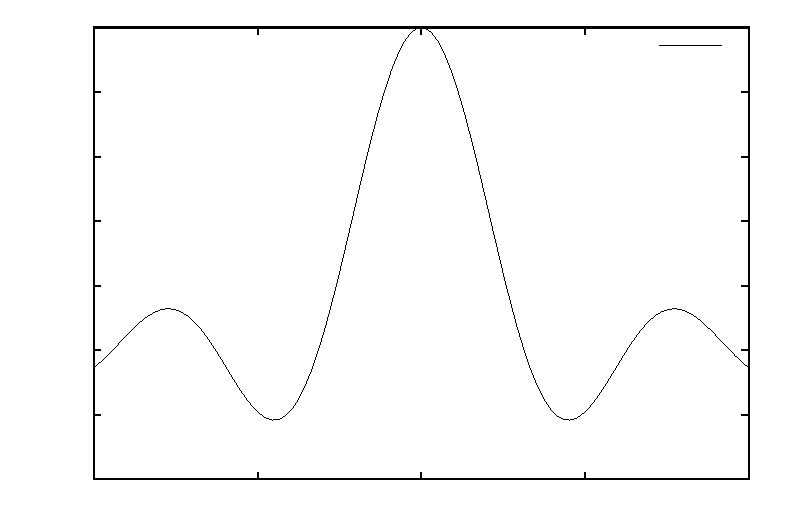
\includegraphics{function_small}}%
    \gplfronttext
  \end{picture}%
\endgroup
}
{Grafico della funzione (\ref{eq:FunzioneGnuplot}), prodotto
da \gnuplot\ con il semplice comando \cchar{plot sin(x)/x}.}
{fig:FunzioneGnuplot}

\noindent Teniamo a mente il comando \cchar{plot}, che abbiamo appena
utilizzato, perch\'e si tratta di uno dei comandi fondamentali e lo
incontreremo ancora sovente, nel seguito.

Trovandoci a parlare di funzioni, notiamo subito come \gnuplot\
supporti in modo estensivo essenzialmente tutte le funzioni con cui si ha a
che fare di solito nell'analisi di dati scientifici (queste includono, ma non
sono limitate a, funzioni trigonometriche, esponenziali e logaritmi).
Se siete incerti su come si possa scrivere il nome di una funzione in modo
che \gnuplot\ \emph{capisca} che cosa volete dire, provate semplicemente a
digitare:
\begin{verbatim}
gnuplot> help functions
\end{verbatim}
ed otterrete tutte le informazioni di cui avete bisogno.
Notiamo anche come le funzioni possano essere poi \emph{combinate}
ulteriormente tra di loro con gli usuali operatori aritmetici che si trovano
elencati in tabella
\ref{tab:OperatoriGnuplot}.

\begin{table}[htbp]
\stdtable{2}%
{Operatore           & Simbolo}%
{Addizione           & \texttt{+}\\
Sottrazione          & \texttt{-}\\
Moltiplicazione      & \texttt{*}\\
Divisione            & \texttt{/}\\
Elevamento a potenza & \texttt{**}\\
}
\caption{Associazione tra gli operatori aritmetici di base ed il simbolo
corrispondente all'interno della \emph{shell} di \gnuplot.}
\label{tab:OperatoriGnuplot}
\end{table}

Spulciando tra le funzioni disponibili all'interno di \gnuplot\ troviamo
anche, come era logico aspettarsi, la \emph{error function} che abbiamo
introdotto a proposito della distribuzione di Gauss e che si trova descritta
in dettaglio in appendice \ref{app:Erf} e tabulata nelle appendici
\ref{app:Erf1} e \ref{app:Erf2}.
In effetti possiamo leggere direttamente dalle tavole (cfr. \ref{app:Erf1}):
$$
\erf(1) = 0.3413
$$
Proviamo allora ad ottenere lo stesso risultato utilizzando \gnuplot; per far
questo ci servir\`a, come vedremo, il comando \cchar{print}, che
sostanzialmente consente di stampare sullo schermo%
\footnote{
Ad essere rigorosi questo non \`e necessariamente vero. Volendo, l'uscita del
comando print pu\`o essere rediretta su un \emph{file} attraverso l'apposito
comando \cchar{set print}.
}
il valore di un'espressione, passata come argomento. Digitiamo:
\begin{verbatim}
gnuplot> print erf(1)
0.842700790029219
\end{verbatim}
Vi \`e chiaramente qualcosa che non va, perch\'e il numero che otteniamo non
\`e corretto. Ma se leggiamo attentamente il contenuto dell'appendice
\ref{app:Erf}, vi troviamo un esplicito riferimento al fatto che ci sono due
definizioni differenti della \emph{error function}, $\erf(x)$ ed $\Erf(x)$,
legate dalla relazione:
$$
\erf(x) = \frac{1}{2} \Erf \left( \frac{x}{\sqrt{2}} \right)
$$
Nelle tavole numeriche noi utilizziamo la prima, ma potrebbe darsi che
\gnuplot\ usi l'altra. Proviamo allora a digitare:
\begin{verbatim}
gnuplot> print 0.5*erf(1/sqrt(2))
0.341344745680573
\end{verbatim}
Questa volta abbiamo il risultato corretto, il che conferma la nostra ipotesi.
Notiamo per inciso che, sebbene non costituisca il modo pi\`u efficiente,
il comando \cchar{print} permette, in linea di principio, di rigenerare le
tavole numeriche riportate nelle sopracitate appendici.
Pi\`u semplicemente, esso permette di evitare l'interpolazione tra valori
tabulati, ogni qual volta si abbia un calcolatore a disposizione.


\section{\ldots e due cose meno ovvie}

Vi sono situazioni in cui il calcolatore sembra fornire all'utente dei
risultati inaspettati, apparentemente errati, o addirittura assurdi.
Lo scopo dichiarato di questo paragrafo \`e di mostrare come, nella stragrande
maggioranza di questi casi, non sia il computer a sbagliare; pi\`u
semplicemente l'utilizzatore ha posto al computer una domanda che \`e
effettivamente \emph{diversa} da quella che egli stesso, in buona fede,
credeva aver posto.
Si pu\`o dire, a buon diritto, che in questa difficolt\`a di comunicazione
tra utente e calcolatore risieda l'origine di un gran parte degli errori di
programmazione. Che \`e come dire che, una volta pensata una \emph{domanda}
che si vuol porre al calcolatore, il punto fondamentale \`e formularla in
modo corretto nel linguaggio del calcolatore stesso.

Supponiamo dunque di voler disegnare il grafico della funzione
(\ref{eq:FunzioneGnuplot}) in un intervallo specifico della variabile
indipendente $x$. Per fissare li idee, supponiamo che questo intervallo
sia $\cinterval{-170}{170}$.
Vi \`e un comando specifico, \cchar{set xrange}, per fissare i limiti di
variabilit\`a della $x$, per cui proveremo a scrivere:
\begin{verbatim}
gnuplot> set xrange [-170:170]
gnuplot> plot sin(x)/x
\end{verbatim}
Il risultato, che \`e mostrato in figura \ref{fig:FunzioneGnuplotLarga},
non pu\`o non destare perplessit\`a.
\panelfig
{% GNUPLOT: LaTeX picture with Postscript
\begingroup
\footnotesize
  \makeatletter
  \providecommand\color[2][]{%
    \GenericError{(gnuplot) \space\space\space\@spaces}{%
      Package color not loaded in conjunction with
      terminal option `colourtext'%
    }{See the gnuplot documentation for explanation.%
    }{Either use 'blacktext' in gnuplot or load the package
      color.sty in LaTeX.}%
    \renewcommand\color[2][]{}%
  }%
  \providecommand\includegraphics[2][]{%
    \GenericError{(gnuplot) \space\space\space\@spaces}{%
      Package graphicx or graphics not loaded%
    }{See the gnuplot documentation for explanation.%
    }{The gnuplot epslatex terminal needs graphicx.sty or graphics.sty.}%
    \renewcommand\includegraphics[2][]{}%
  }%
  \providecommand\rotatebox[2]{#2}%
  \@ifundefined{ifGPcolor}{%
    \newif\ifGPcolor
    \GPcolorfalse
  }{}%
  \@ifundefined{ifGPblacktext}{%
    \newif\ifGPblacktext
    \GPblacktexttrue
  }{}%
  % define a \g@addto@macro without @ in the name:
  \let\gplgaddtomacro\g@addto@macro
  % define empty templates for all commands taking text:
  \gdef\gplbacktext{}%
  \gdef\gplfronttext{}%
  \makeatother
  \ifGPblacktext
    % no textcolor at all
    \def\colorrgb#1{}%
    \def\colorgray#1{}%
  \else
    % gray or color?
    \ifGPcolor
      \def\colorrgb#1{\color[rgb]{#1}}%
      \def\colorgray#1{\color[gray]{#1}}%
      \expandafter\def\csname LTw\endcsname{\color{white}}%
      \expandafter\def\csname LTb\endcsname{\color{black}}%
      \expandafter\def\csname LTa\endcsname{\color{black}}%
      \expandafter\def\csname LT0\endcsname{\color[rgb]{1,0,0}}%
      \expandafter\def\csname LT1\endcsname{\color[rgb]{0,1,0}}%
      \expandafter\def\csname LT2\endcsname{\color[rgb]{0,0,1}}%
      \expandafter\def\csname LT3\endcsname{\color[rgb]{1,0,1}}%
      \expandafter\def\csname LT4\endcsname{\color[rgb]{0,1,1}}%
      \expandafter\def\csname LT5\endcsname{\color[rgb]{1,1,0}}%
      \expandafter\def\csname LT6\endcsname{\color[rgb]{0,0,0}}%
      \expandafter\def\csname LT7\endcsname{\color[rgb]{1,0.3,0}}%
      \expandafter\def\csname LT8\endcsname{\color[rgb]{0.5,0.5,0.5}}%
    \else
      % gray
      \def\colorrgb#1{\color{black}}%
      \def\colorgray#1{\color[gray]{#1}}%
      \expandafter\def\csname LTw\endcsname{\color{white}}%
      \expandafter\def\csname LTb\endcsname{\color{black}}%
      \expandafter\def\csname LTa\endcsname{\color{black}}%
      \expandafter\def\csname LT0\endcsname{\color{black}}%
      \expandafter\def\csname LT1\endcsname{\color{black}}%
      \expandafter\def\csname LT2\endcsname{\color{black}}%
      \expandafter\def\csname LT3\endcsname{\color{black}}%
      \expandafter\def\csname LT4\endcsname{\color{black}}%
      \expandafter\def\csname LT5\endcsname{\color{black}}%
      \expandafter\def\csname LT6\endcsname{\color{black}}%
      \expandafter\def\csname LT7\endcsname{\color{black}}%
      \expandafter\def\csname LT8\endcsname{\color{black}}%
    \fi
  \fi
  \setlength{\unitlength}{0.0500bp}%
  \begin{picture}(7560.00,5040.00)%
    \gplgaddtomacro\gplbacktext{%
      \csname LTb\endcsname%
      \put(770,440){\makebox(0,0)[r]{\strut{}-0.2}}%
      \put(770,982){\makebox(0,0)[r]{\strut{}-0.1}}%
      \put(770,1524){\makebox(0,0)[r]{\strut{} 0}}%
      \put(770,2066){\makebox(0,0)[r]{\strut{} 0.1}}%
      \put(770,2608){\makebox(0,0)[r]{\strut{} 0.2}}%
      \put(770,3150){\makebox(0,0)[r]{\strut{} 0.3}}%
      \put(770,3692){\makebox(0,0)[r]{\strut{} 0.4}}%
      \put(770,4234){\makebox(0,0)[r]{\strut{} 0.5}}%
      \put(770,4776){\makebox(0,0)[r]{\strut{} 0.6}}%
      \put(1272,220){\makebox(0,0){\strut{}-150}}%
      \put(2196,220){\makebox(0,0){\strut{}-100}}%
      \put(3120,220){\makebox(0,0){\strut{}-50}}%
      \put(4044,220){\makebox(0,0){\strut{} 0}}%
      \put(4968,220){\makebox(0,0){\strut{} 50}}%
      \put(5892,220){\makebox(0,0){\strut{} 100}}%
      \put(6816,220){\makebox(0,0){\strut{} 150}}%
    }%
    \gplgaddtomacro\gplfronttext{%
      \csname LTb\endcsname%
      \put(6199,4603){\makebox(0,0)[r]{\strut{}sin(x)/x}}%
    }%
    \gplbacktext
    \put(0,0){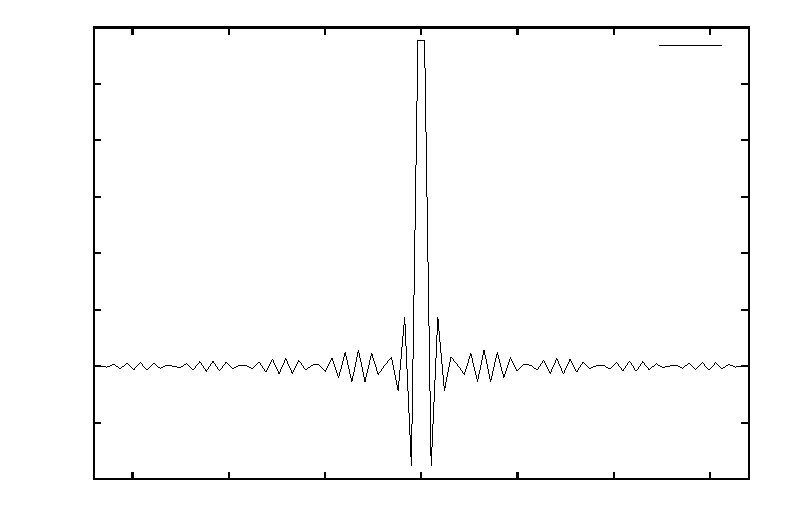
\includegraphics{function_large}}%
    \gplfronttext
  \end{picture}%
\endgroup
}
{Grafico della funzione (\ref{eq:FunzioneGnuplot}), prodotto
da \gnuplot, nell'intervallo $\cinterval{-170}{170}$.}
{fig:FunzioneGnuplotLarga}
Sicuramente il gran numero di cuspidi confligge palesemente con il fatto ben
noto che la funzione \`e in effetti derivabile su tutta la retta reale.
Eppure ci\`o che abbiamo fatto \`e cos\`i semplice (si tratta in fondo di due
soli comandi) e naturale che non \`e ovvio, a prima vista, il punto esatto in
cui abbiamo sbagliato.

La questione ci riporta per un attimo indietro ad analizzare pi\`u in dettaglio
il comando \cchar{plot}. La domanda che ci facciamo \`e, in altre parole:
che cosa fa effettivamente \gnuplot\ quando noi impartiamo un comando
\cchar{plot}?
Beh, per dirla in breve, essenzialmente divide l'intervallo di variabilit\`a
della variabile indipendente $x$%
\footnote{
Se non dichiariamo esplicitamente questo intervallo, \gnuplot\ lo sceglie da
solo, preliminarmente.
}
in un certo numero di intervalli, calcola il valore della funzione in
corrispondenza degli estremi di questi intervalli (in termini tecnici si dice
che \emph{campiona} la funzione) e quindi unisce con delle spezzate
i valori calcolati. Questo ci suggerisce che l'aspetto del grafico in figura
\ref{fig:FunzioneGnuplotLarga} possa essere in effetti dovuto ad un semplice
problema di visualizzazione, connesso con il fatto che abbiamo campionato la
funzione in modo troppo grossolano.

Leggendo la documentazione impariamo che, di \emph{default}, il numero di
di punti in cui una funzione \`e campionata per il grafico \`e
esattamente $100$. Questo numero pu\`o, come ogni altra cosa, essere
modificata dall'utente; maggiore \`e il numero di punti richiesti, pi\`u lungo
il tempo necessario per la visualizzazione, come \`e logico aspettarsi.
Ad ogni modo il comando specifico per questa operazione \`e
\cchar{set samples}, che accetta come argomento il numero di campionamenti.
Possiamo allora provare:
\begin{verbatim}
gnuplot> set samples 10000
gnuplot> set xrange [-170:170]
gnuplot> plot sin(x)/x
\end{verbatim}
ed il risultato, finalmente ragionevole, \`e mostrato in figura
\ref{fig:FunzioneGnuplotSamples}.
\panelfig
{% GNUPLOT: LaTeX picture with Postscript
\begingroup
\footnotesize
  \makeatletter
  \providecommand\color[2][]{%
    \GenericError{(gnuplot) \space\space\space\@spaces}{%
      Package color not loaded in conjunction with
      terminal option `colourtext'%
    }{See the gnuplot documentation for explanation.%
    }{Either use 'blacktext' in gnuplot or load the package
      color.sty in LaTeX.}%
    \renewcommand\color[2][]{}%
  }%
  \providecommand\includegraphics[2][]{%
    \GenericError{(gnuplot) \space\space\space\@spaces}{%
      Package graphicx or graphics not loaded%
    }{See the gnuplot documentation for explanation.%
    }{The gnuplot epslatex terminal needs graphicx.sty or graphics.sty.}%
    \renewcommand\includegraphics[2][]{}%
  }%
  \providecommand\rotatebox[2]{#2}%
  \@ifundefined{ifGPcolor}{%
    \newif\ifGPcolor
    \GPcolorfalse
  }{}%
  \@ifundefined{ifGPblacktext}{%
    \newif\ifGPblacktext
    \GPblacktexttrue
  }{}%
  % define a \g@addto@macro without @ in the name:
  \let\gplgaddtomacro\g@addto@macro
  % define empty templates for all commands taking text:
  \gdef\gplbacktext{}%
  \gdef\gplfronttext{}%
  \makeatother
  \ifGPblacktext
    % no textcolor at all
    \def\colorrgb#1{}%
    \def\colorgray#1{}%
  \else
    % gray or color?
    \ifGPcolor
      \def\colorrgb#1{\color[rgb]{#1}}%
      \def\colorgray#1{\color[gray]{#1}}%
      \expandafter\def\csname LTw\endcsname{\color{white}}%
      \expandafter\def\csname LTb\endcsname{\color{black}}%
      \expandafter\def\csname LTa\endcsname{\color{black}}%
      \expandafter\def\csname LT0\endcsname{\color[rgb]{1,0,0}}%
      \expandafter\def\csname LT1\endcsname{\color[rgb]{0,1,0}}%
      \expandafter\def\csname LT2\endcsname{\color[rgb]{0,0,1}}%
      \expandafter\def\csname LT3\endcsname{\color[rgb]{1,0,1}}%
      \expandafter\def\csname LT4\endcsname{\color[rgb]{0,1,1}}%
      \expandafter\def\csname LT5\endcsname{\color[rgb]{1,1,0}}%
      \expandafter\def\csname LT6\endcsname{\color[rgb]{0,0,0}}%
      \expandafter\def\csname LT7\endcsname{\color[rgb]{1,0.3,0}}%
      \expandafter\def\csname LT8\endcsname{\color[rgb]{0.5,0.5,0.5}}%
    \else
      % gray
      \def\colorrgb#1{\color{black}}%
      \def\colorgray#1{\color[gray]{#1}}%
      \expandafter\def\csname LTw\endcsname{\color{white}}%
      \expandafter\def\csname LTb\endcsname{\color{black}}%
      \expandafter\def\csname LTa\endcsname{\color{black}}%
      \expandafter\def\csname LT0\endcsname{\color{black}}%
      \expandafter\def\csname LT1\endcsname{\color{black}}%
      \expandafter\def\csname LT2\endcsname{\color{black}}%
      \expandafter\def\csname LT3\endcsname{\color{black}}%
      \expandafter\def\csname LT4\endcsname{\color{black}}%
      \expandafter\def\csname LT5\endcsname{\color{black}}%
      \expandafter\def\csname LT6\endcsname{\color{black}}%
      \expandafter\def\csname LT7\endcsname{\color{black}}%
      \expandafter\def\csname LT8\endcsname{\color{black}}%
    \fi
  \fi
  \setlength{\unitlength}{0.0500bp}%
  \begin{picture}(7560.00,5040.00)%
    \gplgaddtomacro\gplbacktext{%
      \csname LTb\endcsname%
      \put(770,440){\makebox(0,0)[r]{\strut{}-0.4}}%
      \put(770,1059){\makebox(0,0)[r]{\strut{}-0.2}}%
      \put(770,1679){\makebox(0,0)[r]{\strut{} 0}}%
      \put(770,2298){\makebox(0,0)[r]{\strut{} 0.2}}%
      \put(770,2918){\makebox(0,0)[r]{\strut{} 0.4}}%
      \put(770,3537){\makebox(0,0)[r]{\strut{} 0.6}}%
      \put(770,4157){\makebox(0,0)[r]{\strut{} 0.8}}%
      \put(770,4776){\makebox(0,0)[r]{\strut{} 1}}%
      \put(1272,220){\makebox(0,0){\strut{}-150}}%
      \put(2196,220){\makebox(0,0){\strut{}-100}}%
      \put(3120,220){\makebox(0,0){\strut{}-50}}%
      \put(4044,220){\makebox(0,0){\strut{} 0}}%
      \put(4968,220){\makebox(0,0){\strut{} 50}}%
      \put(5892,220){\makebox(0,0){\strut{} 100}}%
      \put(6816,220){\makebox(0,0){\strut{} 150}}%
    }%
    \gplgaddtomacro\gplfronttext{%
      \csname LTb\endcsname%
      \put(6199,4603){\makebox(0,0)[r]{\strut{}sin(x)/x}}%
    }%
    \gplbacktext
    \put(0,0){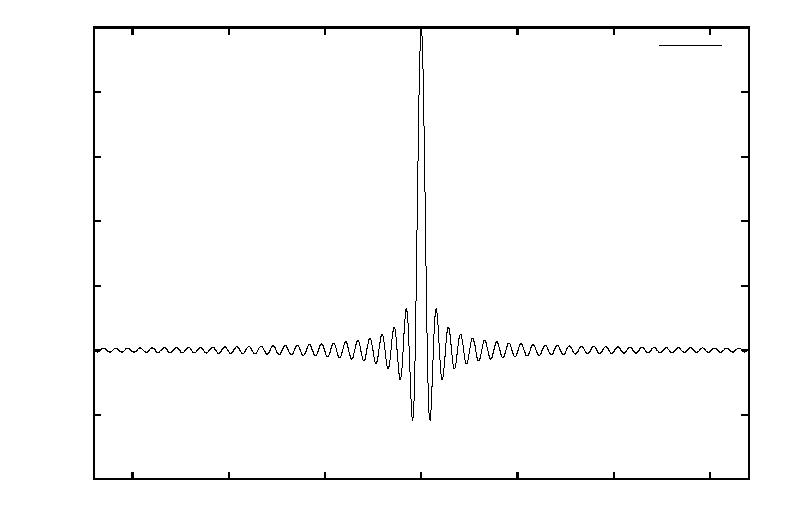
\includegraphics{function_sampled}}%
    \gplfronttext
  \end{picture}%
\endgroup
}
{Grafico della funzione (\ref{eq:FunzioneGnuplot}), prodotto
da \gnuplot, nell'intervallo $\cinterval{-170}{170}$, con un numero
di punti di campionamento pari a $10000$.}
{fig:FunzioneGnuplotSamples}

Torniamo allora per un istante a quanto detto all'inizio del paragrafo e
cerchiamo di interpretare i due ultimi grafici nel nostro nuovo schema
concettuale. In buona fede eravamo convinti di chiedere al computer di
disegnare il grafico di una funzione; in realt\`a: nel primo caso gli abbiamo
chiesto  di campionare la funzione in $100$ punti e di unire i valori ottenuti
con linee rette, mentre nel secondo gli abbiamo chiesto di fare lo stesso
campionando in $10000$ punti.
In entrambi i casi il calcolatore ha eseguito gli ordini alla lettera; il fatto
che il primo grafico non ci piaccia, mentre il secondo sia esteticamente
appagante dipende solo da noi.

Avevamo promesso esattamente \emph{due} cose meno ovvie nel titolo del
paragrafo ed ecco qui la seconda. Proviamo a digitare nella \emph{shell}
di \gnuplot\ il comando \cchar{print 1/2}.
Riuscite ad immaginare che cosa succeder\`a? Ebbene, il risultato \`e,
ancora una volta, sorprendente:
\begin{verbatim}
gnuplot> print 1/2
0
\end{verbatim}
Senza perdere troppo tempo, il punto fondamentale \`e che \gnuplot\ interpreta
numeratore e denominatore come numeri interi e restituisce pure il risultato
della divisione come intero (in effetti $0$ \`e la parte intera di
$\frac{1}{2}$).
Si tratta di una \emph{trappola} tipica in cui tutti sono caduti almeno una
volta nella vita ed \`e questo il motivo per cui l'abbiamo mostrata qui.
Se adesso rendiamo manifestamente reali il numeratore ed il denominatore,
tutto torna come ci aspettiamo:
\begin{verbatim}
gnuplot> print 1.0/2.0
0.5
\end{verbatim} 


\section{Visualizzare una serie di dati}

\gnuplot\ \`e capace di visualizzare in modo molto semplice i dati contenuti
in un \emph{file}, purch\'e organizzati per colonne e separati con spazi o
\ckey{TAB}.
Tutte le linee che cominciano con un cancelletto (\cchar{\#}) sono
automaticamente ignorate da \gnuplot\ (e tecnicamente prendono il nome di
\emph{commenti}). Questo permette, tra le altre cose, di inserire in un
generico \emph{file} di dati una breve descrizione del contenuto delle
colonne, di modo che esso sia pi\`u facilmente comprensibile. 

Supponiamo ad esempio di avere un \emph{file} di testo (denominato
\cchar{LeggeOraria.txt}) del tipo:
\begin{verbatim}
# Tempo (sec)   Posizione (cm)   Errore (cm)
5               10.1             2.0
10              17.8             1.5
15              26.6             1.5
20              32.8             2.0
25              40.2             2.5
30              47.4             2.0
\end{verbatim}
Il comando:
\begin{verbatim}
gnuplot> plot 'LeggeOraria.txt' using 1:2
\end{verbatim}
dovrebbe generare qualcosa di non troppo diverso dalla figura
\ref{fig:LeggeOraria}.
\panelfig
{\includegraphics[height=\figwidth, angle=270]%
{./ps_gnuplot/figure/LeggeOraria}}
{Visualizzazione, mediante \gnuplot, dei dati contenuti nel \emph{file}
\cchar{LeggeOraria.txt} (riportato poche righe sopra).}
{fig:LeggeOraria}
In questo contesto il comando \cchar{plot} accetta come argomento il
nome del \emph{file} di testo contenente i dati (racchiuso tra virgolette o
apici) e l'opzione \cchar{using} specifica le colonne che saranno
graficate sull'asse delle $x$ e su quello delle $y$, rispettivamente.
Si tratta di una sintassi tipica che useremo spesso; sottolineiamo anche
esplicitamente il fatto che il comando \cchar{plot} supporta una notevole
quantit\`a di opzioni, come si pu\`o facilmente verificare digitando
\cchar{help plot}.

\caution{\`E molto frequente, specialmente all'inizio, far confusione tra
percorsi relativi ed assoluti ai \emph{file}. Quando scriviamo
\cchar{plot 'LeggeOraria.txt'} assumiamo implicitamente che un \emph{file}
denominato \cchar{LeggeOraria.txt} sia presente nella \emph{directory}
corrente.}

\caution{Se non abbiamo mai usato il comando \cchar{cd} all'interno della
\emph{shell} di \gnuplot, la \emph{directory} corrente sar\`a la
\emph{directory} da cui abbiamo lanciato il programma.
In ogni caso essa pu\`o essere visualizzata tramite il comando \cchar{pwd},
anche questo da digitare nella \emph{shell} di \gnuplot.}

Quando cerchiamo di accedere ad un file che fisicamente non esiste
(o che non si trova nella posizione esatta cui stiamo puntando
all'interno del \emph{filesystem}) otteniamo in generale un messaggio d'errore.
Tanto per fissare le idee, supponiamo di aver lanciato \gnuplot\ da una certa
\emph{directory} e di avere il \emph{file} di dati \cchar{LeggeOraria.txt}
all'interno di una \emph{directory} denominata \cchar{dati} e situata a sua
volta all'interno della \emph{directory} di partenza.
Digitando il comando precedente provocheremo ovviamente un errore:
\begin{verbatim}
gnuplot> plot 'LeggeOraria.txt' using 1:2
              ^
         can't read data file "LeggeOraria.txt"
           
\end{verbatim}
perch\'e \gnuplot\ non trover\`a fisicamente il \emph{file}. Abbiamo allora
due possibilit\`a distinte: scrivere il percorso completo al \emph{file}:
\begin{verbatim}
gnuplot> plot './data/LeggeOraria.txt' using 1:2
\end{verbatim}
oppure cambiare \emph{directory} e successivamente impartire il comando
\cchar{plot}:
\begin{verbatim}
gnuplot> cd './data'
gnuplot> plot 'LeggeOraria.txt' using 1:2
\end{verbatim}

\caution{Il lettore non deve far confusione tra il comando \cchar{cd} di
\gnuplot\ ed il comando standard \ccmd{cd} di \linux. In particolare il primo
richiede che il nome della \emph{directory} di destinazione sia racchiuso
tra virgolette o apici.}

Ogni volta che si ha un messaggio di errore del tipo
\cchar{can't read data file \ldots} significa che, in un modo o nell'altro,
stiamo puntando ad un \emph{file} che fisicamente non si trova dove noi
pensiamo (o che magari non ci siamo nemmeno posti il problema).
In tal caso le cose da fare sono due: capire dove siamo
con il comando \cchar{pwd} (da digitare nella \emph{shell} di \gnuplot) e
quindi indirizzare il \emph{file} correttamente in uno dei due modi appena
mostrati.

Torniamo adesso alla nostra serie di dati e vediamo brevemente alcuni comandi
specifici di formattazione dei grafici. Supponiamo di digitare, nella
\emph{shell} di \gnuplot:
\begin{verbatim}
gnuplot> set title 'Legge oraria per una particella libera'
gnuplot> set xlabel 'Tempo (sec)'
gnuplot> set ylabel 'Posizione (cm)'
gnuplot> set xrange [0: 40]
gnuplot> set yrange [0: 50]
gnuplot> unset key
gnuplot> plot 'LeggeOraria.txt' using 1:2:3 with yerrorbars
\end{verbatim}
Il risultato \`e mostrato in figura \ref{fig:LeggeOrariaEdit}.
\panelfig
{\includegraphics[height=\figwidth, angle=270]%
{./ps_gnuplot/figure/LeggeOrariaEdit}}
{Visualizzazione, mediante \gnuplot, dei dati contenuti nel \emph{file}
\cchar{LeggeOraria.txt}, dopo alcuni semplici comandi di formattazione.}
{fig:LeggeOrariaEdit}
La maggior parte dei nuovi comandi introdotti dovrebbe essere auto-esplicativa.
In particolare dovrebbe essere chiaro come inserire il titolo del grafico,
impostare gli estremi dei due assi e mettere delle \emph{etichette} di testo
(in inglese si chiamano \emph{label}) sugli assi stessi.
Pur tuttavia commenteremo esplicitamente gli ultimi due. Il primo:
\begin{verbatim}
gnuplot> unset key
\end{verbatim}
sostanzialmente elimina la legenda, che altrimenti viene inserita nel grafico
in alto a destra (cfr. figura \ref{fig:LeggeOraria}). L'altro \`e l'usuale
comando \cchar{plot}:
\begin{verbatim}
gnuplot> plot 'LeggeOraria.txt' using 1:2:3 with yerrorbars
\end{verbatim}
che viene per\`o usato, questa volta, con l'opzione \cchar{with yerrorbars},
la quale permette di rappresentare sul grafico le barre d'errore sull'asse
delle $y$; la colonna dei valori per le barre d'errore viene passata come
terzo argomento dell'opzione \cchar{using}.
Esiste anche un'opzione \cchar{with xyerrorbars} che permette di rappresentare
le barre d'errore su entrambi gli assi; in questo caso le quattro colonne che
sono passate all'opzione \cchar{using} sono interpretate come $x$, $y$,
$\Delta x$ e $\Delta y$, rispettivamente.

\caution{Tutti i comandi di formattazione hanno effetto solamente nel momento
in cui si impartisce un nuovo comando \cchar{plot} e non prima; di converso il
loro effetto cessa solamente nel momento in cui vengono esplicitamente
sovrascritti oppure quando si esce da \gnuplot. Vale anche la pena di
menzionare il comando \cchar{replot} il quale non fa altro che ripetere
esattamente l'ultimo comando \cchar{plot}.}


\section{Realizzare un istogramma}

Diciamo subito che \gnuplot\ \emph{non} supporta la realizzazione di
istogrammi, nel senso che non ha le funzionalit\`a per creare i canali e
popolarli a partire da una serie di dati.
Pur tuttavia esiste un'opzione di \emph{visualizzazione} del comando
\cchar{plot} dedicata specificamente alla creazione istogrammi%
\footnote{
Sottolineiamo esplicitamente che si tratta solo di un opzione di
visualizzazione e che la definizione ed il popolamento dei canali debbono
essere eseguiti dall'utente.
}%
.
Senza entrare troppo nei dettagli diremo che se forniamo a \gnuplot\ un
\emph{file} di dati (supponiamo, per fissare le idee, che si chiami
\cchar{Istogramma.txt}) contenente una colonna con le coordinate
centrali dei canali ed una con il contenuto dei canali stessi, possiamo
disegnare l'istogramma corrispondente con un comando del tipo:
\begin{verbatim}
gnuplot> plot 'Istogramma.txt' using 1:2 with histeps
\end{verbatim}



\section{Salvare i grafici sotto forma di immagini}

Il lettore potr\`a chiedersi come sia stato possibile salvare i grafici
generati da \gnuplot\ in una forma che permettesse di inserirli nel paragrafo
precedente (e precisamente sotto forma di \emph{file} postscript).
Prima di mostrare esplicitamente i comandi che serviranno \`e tuttavia
necessario introdurre due concetti nuovi di fondamentale importanza:
\begin{numlist}
\item{
\cchar{output}:
\`e sostanzialmente il luogo in cui vengono mostrate (o, pi\`u precisamente
\emph{redirette}) le schermate di \gnuplot\ (in Italiano diremmo
\emph{uscita}). Nel nostro caso esso pu\`o essere, a seconda dei casi, il
monitor del calcolatore oppure un \emph{file}%
\footnote{
Vi sono in effetti alcune altre possibilit\`a un poco pi\`u esotiche che
potete trovare nella documentazione specifica.
}%
.
Vedremo tra breve come passare da una modalit\`a all'altra.
}
\item{
\cchar{terminal}:
\`e il \emph{linguaggio} con cui le schermate di \gnuplot\ vengono redirette
sull'uscita (qualunque essa sia). Nel caso l'uscita sia un \emph{file}, questo
linguaggio pu\`o essere, ad esempio postscript, gif, png, etc.
Nel caso in cui invece vogliamo, come accade tipicamente, le schermate
sul monitor, questo linguaggio sar\`a, in un qualche senso, il
linguaggio del sistema operativo; come vedremo nel seguito, il nome da usare
sar\`a \cchar{x11} sotto \linux\ e \cchar{windows} sotto \windows.
}
\end{numlist}

A questo punto non dovrebbe essere troppo difficile capire come si possa
salvare un grafico sotto forma di immagine: dovremo redirigere l'uscita su di
un \emph{file} specifico ed impostare opportunamente il terminale.
Vale a dire qualcosa del genere:
\begin{verbatim}
gnuplot> set terminal postscript
gnuplot> set output 'Immagine.eps'
gnuplot> replot
gnuplot> set output
gnuplot> set terminal x11
\end{verbatim}

\caution{I comandi \cchar{set output} e \cchar{set terminal} non sono
indipendenti l'uno dall'altro: non tutti i terminali sono appropriati per
tutti i tipi di \emph{output} e viceversa.
Il lettore potr\`a divertirsi, per curiosit\`a, a provare alcune delle
combinazioni \emph{proibite} (come terminale postscript su \emph{output}
standard oppure terminale \cchar{x11} su di un \emph{file}).
Gli effetti saranno interessanti.}

Analizziamo i comandi appena scritti uno per uno, alla luce di quanto detto
sino ad ora. I primi due
\begin{verbatim}
gnuplot> set terminal postscript
gnuplot> set output 'Immagine.eps'
\end{verbatim}
redirigono l'uscita su di una \emph{file} che si chiamer\`a
\cchar{Immagine.eps}%
\footnote{
Se non specifichiamo il percorso completo il \emph{file} verr\`a creato nella
\emph{directory} corrente. \`E importante anche notare che, nel caso esista
gi\`a un \emph{file} con lo stesso nome, esso verr\`a sovrascritto senza che ne
venga richiesta conferma.
}
e che verr\`a scritto in linguaggio postscript, come specificato nella
impostazione del terminale.
Il comando successivo:
\begin{verbatim}
gnuplot> replot
\end{verbatim}
esegue di nuovo l'ultimo comando plot che \`e stato digitato. In questo caso,
essendo l'\emph{output} rediretto su \emph{file}, il grafico non apparir\`a
sullo schermo; al contrario verr\`a fisicamente \emph{scritto} sul \emph{file}
stesso. Quando torniamo sull'\emph{output} standard, vale a dire sullo schermo
del calcolatore:
\begin{verbatim}
gnuplot> set output
\end{verbatim}
il \emph{file} di uscita viene \emph{chiuso}. L'ultimo comando permette di
impostare di nuovo il terminale nella modalit\`a di default:
\begin{verbatim}
gnuplot> set terminal x11
\end{verbatim}
e siamo di nuovo al punto di partenza, in cui i comandi \cchar{plot} producono
bellissimi grafici sullo schermo. Vale la pena notare che, se lavorassimo sotto
\windows, quest'ultimo comando (e solo questo) sarebbe diverso:
\begin{verbatim}
gnuplot> set terminal windows
\end{verbatim}


\section{Il concetto di macro}

Adesso che il nostro vocabolario, in termini di comandi di \gnuplot, si \`e
fatto abbastanza ampio da consentirci di produrre una certa quantit\`a di cose
interessanti, diventa davvero indispensabile introdurre il concetto di
\emph{macro}. In termini semplici una macro \`e una sequenza di comandi
(validi) inseriti, uno dopo l'altro, in un \emph{file} di testo.
Il vantaggio fondamentale del lavorare con le macro \`e che, mentre tutti i
comandi che digitiamo nel prompt vanno perduti non appena usciamo dal
programma, una macro, una volta salvata, pu\`o essere riutilizzata
(eventualmente dopo modifiche) a distanza di tempo. Come vedremo, \`e
sufficiente un solo comando per eseguirla.

Una tipica macro che utilizzi i comandi imparati sino ad ora potrebbe apparire
come segue:
\begin{verbatim}
# Inizializzazione.
set output
set terminal x11

# Definizione e formattazione del grafico.
set title 'Legge oraria per una particella libera'
set xlabel 'Tempo (sec)'
set ylabel 'Posizione (cm)'
set xrange [0: 40]
set yrange [0: 50]
unset key
plot 'LeggeOraria.txt' using 1:2:3 with yerrorbars

# Creazione del file di uscita.
set terminal postscript
set output 'Immagine.eps'
replot

# Ritorno allo schermo.
set output
set terminal x11
\end{verbatim}

Dato che, come gi\`a sappiamo, le linee che cominciano con un cancelletto
vengono ignorate da \gnuplot, nella macro qui sopra ne abbiamo usate alcune per
commentare la macro stessa. Si tratta di una buona abitudine che, unita all'uso
di linee vuote per separare blocchi logici distinti, aumenta la
leggibilit\`a.
Notiamo esplicitamente come i primi due comandi:
\begin{verbatim}
gnuplot> set output
gnuplot> set terminal x11
\end{verbatim}
pur se non formalmente necessari, costituiscano pure una buona abitudine,
che pu\`o salvare da apparenti inconsistenze nel caso in cui le impostazioni
di partenza non siano, per qualche ragione, quelle che ci aspettiamo. 

Supponendo dunque che il \emph{file} di testo in cui abbiamo salvato la macro
si chiami \cchar{macro.txt}, essa si esegue digitando nella \emph{shell} di
\gnuplot:
\begin{verbatim}
gnuplot> load 'macro.txt'
\end{verbatim}
Questo dovrebbe produrre sostanzialmente la figura \ref{fig:LeggeOrariaEdit}.


\section{Eseguire un fit ad una serie di dati}

\gnuplot\ permette di eseguire un fit del minimo $\chi^2$ ad una serie di dati%
\footnote{
Per essere precisi, \gnuplot\ utilizza una propria implementazione
dell'algoritmo di Marquardt-Levenberg per il fit non lineare dei minimi
quadrati (NLLS). I punti sono pesati con l'inverso del loro errore, per cui
questo metodo \`e in effetti concettualmente affine a quello che noi
conosciamo come metodo del minimo $\chi^2$.
}
con una generica funzione definita dall'utente. I comandi coinvolti in questa
operazione sono, pi\`u o meno, i seguenti:
\begin{verbatim}
gnuplot> f(x) = a + b*x
gnuplot> a = 1
gnuplot> b = 1
gnuplot> fit f(x) 'LeggeOraria.txt' using 1:2:3 via a, b 
\end{verbatim}
Al solito li analizzeremo brevemente uno ad uno. Il primo:
\begin{verbatim}
gnuplot> f(x) = a + b*x
\end{verbatim}
definisce la funzione con cui vogliamo eseguire il fit. In questo caso \`e
semplicemente una retta, ma si possono utilizzare tutte le funzioni predefinite
in \gnuplot, eventualmente combinate attraverso gli operatori in tabella
\ref{tab:OperatoriGnuplot}. Il che \`e sufficiente per la stragrande
maggioranza delle applicazioni.
I due comandi successivi:
\begin{verbatim}
gnuplot> a = 1
gnuplot> b = 1
\end{verbatim}
inizializzano i parametri della funzione con cui si fa il fit.

\caution{Il modo in cui il calcolatore esegue un fit \`e, per molti aspetti,
\emph{diverso} da come faremmo noi, seguendo i metodi descritti nel capitolo
\ref{chap:fit}. In particolare, anche nei casi in cui le equazioni a cui porta
il metodo del minimo $\chi^2$ si possono risolvere analiticamente, il
calcolatore utilizza dei metodi numerici per cui i valori iniziali dei
parametri sono essenziali. Vi sono casi, nemmeno troppi complicati, in cui il
fit pu\`o convergere o non convergere, a seconda di come inizializziamo i
parametri. Vi sono anche casi, per certi versi ancor pi\`u pericolosi, in cui
valori iniziali diversi fanno convergere il fit a valori finali diversi.
In ogni caso, \`e una buona abitudine fornire una stima sensata dei parametri
(magari solo guardando il grafico) prima di cominciare il fit.}

\noindent L'ultimo comando:
\begin{verbatim}
gnuplot> fit f(x) 'LeggeOraria.txt' using 1:2:3 via a, b
\end{verbatim}
\`e quello che esegue il fit propriamente detto. Esso accetta come parametro la
funzione con cui fittare i dati ed il nome del \emph{file} in cui i dati
stessi sono contenuti.
Le tre colonne che vengono passate all'opzione \cchar{using} sono interpretate
come valori della $x$, della $y$ e degli errori sulla $y$, rispettivamente
La terza colonna (quella degli errori sulla $y$) non \`e strettamente
richiesta.

\caution{Se gli errori sulla $y$ non vengono forniti, \gnuplot\ assume
che essi siano tutti pari ad $1$; questo \`e rilevante (\`e importante
ricordarlo) per il valore del $\chi^2$ che, come vedremo, il fit fornisce
come sottoprodotto); \gnuplot\ \emph{non} supporta fit di tipo generale
(vale a dire con errori su entrambe le variabili).}

\noindent L'opzione \cchar{via} definisce quali tra i parametri della funzione
siano liberi di variare durante il fit (quelli che eventualmente non sono
menzionati sono considerati fissi al loro valore iniziale).

Se le cose non fossero ancora perfettamente chiare, la macro seguente:
\begin{verbatim}
# Inizializzazione.
set output
set terminal x11

# Definizione e formattazione del grafico.
set title 'Legge oraria per una particella libera'
set xlabel 'Tempo (sec)'
set ylabel 'Posizione (cm)'
set xrange [0: 40]
set yrange [0: 50]
unset key

# Esecuzione del fit
f(x) = a + b*x
a = 1
b = 1
fit f(x) 'LeggeOraria.txt' using 1:2:3 via a, b

# Creazione del grafico.
plot 'LeggeOraria.txt' using 1:2:3 with yerrorbars, f(x)

# Creazione del file di uscita.
set terminal postscript
set output 'Immagine.eps'
replot

# Ritorno allo schermo.
set output
set terminal x11
\end{verbatim}
dovrebbe produrre, ammesso che tutto funzioni correttamente, il grafico in
figura
\ref{fig:LeggeOrariaFit}.
\panelfig
{\includegraphics[height=\figwidth, angle=270]%
{./ps_gnuplot/figure/LeggeOrariaFit}}
{Grafico prodotto dalla macro riportata in questa sezione.}
{fig:LeggeOrariaFit}
Notiamo come il comando \cchar{plot} permetta di graficare pi\`u oggetti (in
questo caso una serie di dati ed una funzione), a patto che essi siano separati
da una virgola.

Contestualmente al grafico (mostrato sullo schermo e salvato su di un
\emph{file}) il comando \cchar{fit} produrr\`a una serie di linee sul
terminale di \gnuplot, contenenti informazioni sull'esito del fit stesso%
\footnote{
Queste informazioni sono anche salvate, per futura referenza, su un
\emph{file} di testo chiamato \cchar{fit.log} e salvato nella \emph{directory}
corrente.
}%
:
\begin{verbatim}
***********************************************************
Wed Feb 12 09:45:22 2003


FIT:    data read from 'LeggeOraria.txt' using 1:2:3
        #datapoints = 6
function used for fitting: f(x)
fitted parameters initialized with current variable values



Iteration 0
WSSR        : 209.004           delta(WSSR)/WSSR   : 0
delta(WSSR) : 0                 limit for stopping : 1e-05
lambda    : 6.93718

initial set of free parameter values

a               = 1
b               = 1

After 5 iterations the fit converged.
final sum of squares of residuals : 0.686015
rel. change during last iteration : -2.87956e-12

degrees of freedom (ndf) : 4
rms of residuals      (stdfit) = sqrt(WSSR/ndf)      : 0.41413
variance of residuals (reduced chisquare) = WSSR/ndf : 0.171504

Final set of parameters            Asymptotic Standard Error
=======================            ==========================

a               = 3.25533          +/- 0.698        (21.44%)
b               = 1.48589          +/- 0.03902      (2.626%)


correlation matrix of the fit parameters:

               a      b
a               1.000
b              -0.897  1.000
\end{verbatim}
Le informazioni pi\`u importanti sono i valori finali dei parametri che
si trovano dopo la riga:
\begin{verbatim}
Final set of parameters            Asymptotic Standard Error
=======================            ==========================

a               = 3.25533          +/- 0.698        (21.44%)
b               = 1.48589          +/- 0.03902      (2.626%)
\end{verbatim}
la matrice di correlazione dei parametri, che abbiamo definito nel
paragrafo \ref{sec:Correlazione} e che leggiamo sotto la riga:
\begin{verbatim}
correlation matrix of the fit parameters:

               a      b
a               1.000
b              -0.897  1.000
\end{verbatim}
ed il valore del $\chi^2$ diviso il numero di gradi di libert\`a:
\begin{verbatim}
variance of residuals (reduced chisquare) = WSSR/ndf : 0.171504
\end{verbatim}
Vale la pena di ricordare che, nel caso in cui non si specifichi esplicitamente
una colonna di dati contenente gli errori sulle $y$, il valore del $\chi^2$(che
\gnuplot\ fornisce comunque) perde completamente di significato (in tal caso,
come abbiamo gi\`a detto, il programma assume semplicemente che tutti gli
errori siano pari all'unit\`a).

Come commento finale vorremmo sottolineare che il fatto che il calcolatore
scriva esplicitamente:
\begin{verbatim}
a               = 3.25533          +/- 0.698        (21.44%)
\end{verbatim}
non ci autorizza a dimenticare le regole consuete sulle cifre significative.
Noi scriveremo sempre:
$$
a = 3.25 \pm 0.70
$$


\section{Operazioni con le colonne}

Vi \`e un'ultima cosa che, essendo utile in molte situazioni, vale la pena
di discutere brevemente e si tratta delle operazioni che \gnuplot\ consente
di eseguire con le colonne di un generico \emph{file} di dati.

Supponiamo, per fissare le idee, di avere un \emph{file} di dati (come al
solito organizzato per colonne) e di voler fare un grafico con la colonna
numero $1$ sull'asse delle $x$ ed il \emph{quadrato} della colonna numero $2$
su quello delle $y$. Ebbene, in questo caso scriveremmo:
\begin{verbatim}
gnuplot> plot 'LeggeOraria.txt' using 1:(($2)**2)
\end{verbatim}
Non \`e il caso, di nuovo, di dilungarsi in spiegazioni. Essenzialmente
la scrittura \cchar{(\$2)} identifica la seconda colonna come oggetto nel suo
insieme; dopo di che si pu\`o utilizzare la consueta sintassi (cio\`e le
funzioni e gli operatori che gi\`a conosciamo) per fare operazioni sulle
colonne stesse, elemento per elemento.
A volte, specialmente se le operazioni da fare sulle colonne sono complesse,
se   si vuole vedere il risultato di tali operazioni (quanto meno come
controllo che tutto proceda correttamente) conviene generare un \emph{file} di
dati trasformati (utilizzando un programma che lo consenta, come \scilab) e
quindi lavorare su di essi.
